\documentclass[11pt, a4paper]{article}

% Fonts and Encoding
\usepackage[utf8]{inputenc}
\usepackage[T1]{fontenc}

% Math and Symbols
\usepackage{amsmath, amssymb, amsthm, amsfonts, mathrsfs, mathtools}

% Layout and Geometry
\usepackage{geometry}
\geometry{a4paper, margin=1in}

% Formatting and Graphics
\usepackage{graphicx, xcolor, enumitem, booktabs, array, tabularx}

% TikZ for Illustrations
\usepackage{tikz}
\usetikzlibrary{arrows.meta, positioning, shapes.geometric, calc, backgrounds, matrix}

% Clickable Links and TOC
\usepackage{hyperref}
\hypersetup{
    colorlinks=true,
    linkcolor=blue,
    filecolor=magenta,      
    urlcolor=cyan,
    pdftitle={Advanced Mathematical Induction},
}

% Theorem Environments
\newtheorem{theorem}{Theorem}[section]
\newtheorem{lemma}[theorem]{Lemma}
\newtheorem{proposition}[theorem]{Proposition}
\newtheorem{corollary}[theorem]{Corollary}
\theoremstyle{definition}
\newtheorem{definition}{Definition}[section]
\newtheorem{axiom}{Axiom}[section]
\newtheorem{example}{Example}[section]
\theoremstyle{remark}
\newtheorem{remark}{Remark}[section]

% Custom Commands (Enforced standard notation)
\newcommand{\R}{\mathbb{R}}
\newcommand{\N}{\mathbb{N}}
\newcommand{\Z}{\mathbb{Z}}
\newcommand{\Q}{\mathbb{Q}}
\newcommand{\E}{\mathbb{E}}
\newcommand{\Prob}{\mathbb{P}}
\newcommand{\F}{\mathcal{F}}

\begin{document}

\title{\Huge \textbf{Mastering Mathematical Induction: A Rigorous Foundation} \\ \Large \vspace{10pt} Bridging Abstract Logic to Advanced Quantitative Modeling}
\author{\textbf{Tashfeen Omran}}
\date{\today}

\maketitle
\tableofcontents
\newpage

% ==========================================
% PART 1: INTRODUCTION & CONTEXT
% ==========================================
\section{Comprehensive Introduction, Context, and Prerequisites}

\subsection{Core Concepts \& Axioms}
Mathematical Induction is a foundational proof technique used to establish the truth of an infinite sequence of propositions. While standard induction begins at $n = 1$, Section 6.2 introduces the \textbf{Generalized Principle of Mathematical Induction}. This framework allows the base case to be anchored at any arbitrary integer $m \in \Z$. 

Formally, let $S = \{i \in \Z : i \ge m\}$. If we can prove that a property $P(m)$ holds, and that for any $k \in S$, the truth of $P(k)$ implies the truth of $P(k+1)$, then $P(n)$ is true for all $n \in S$. This relies heavily on the \textbf{Well-Ordering Principle}, which states that every non-empty subset of the natural numbers $\N$ contains a least element.

\subsection{Intuition and Set-Theoretic Foundations}
Intuitively, induction is often compared to an infinite line of falling dominoes. The Generalized Principle simply states that we do not need to start knocking down dominoes at the very first one (index $1$). If we start at index $m$ (which could be negative, zero, or a large positive integer like $10$), and ensure the spacing is such that domino $k$ knocks over domino $k+1$, then all dominoes from $m$ onwards will fall. 

Set-theoretically, induction defines a filter or a truth-set $T = \{n \in S : P(n) \text{ is true}\}$. By proving $m \in T$ and $k \in T \implies k+1 \in T$, we demonstrate that the complement $S \setminus T$ must be empty, forcing $T = S$.

\subsection{Historical Context and Motivation}
The formalization of mathematical induction is deeply tied to the foundational crisis of mathematics in the late 19th and early 20th centuries. Mathematicians like Giuseppe Peano and Richard Dedekind sought to rigorously define the natural numbers. The \textit{Peano Axioms} (specifically the Axiom of Induction) were formulated to prevent logical paradoxes and to provide a rigorous bedrock for arithmetic. As mathematics expanded into abstract algebra and analysis, the need to prove statements for sets starting at arbitrary bounds (e.g., proving inequalities that only hold for $n \ge 10$) necessitated the Generalized Principle.

\subsection{Key Theorems and Lemmas}
\begin{theorem}[Well-Ordering Principle]
Every non-empty subset of $\N$ has a least element.
\end{theorem}

\begin{theorem}[Generalized Principle of Mathematical Induction]
For a fixed integer $m$, let $S = \{i \in \Z : i \ge m\}$. For each $n \in S$, let $P(n)$ be a statement. If:
\begin{enumerate}
    \item $P(m)$ is true, and
    \item $\forall k \in S, P(k) \implies P(k+1)$ is true,
\end{enumerate}
then $P(n)$ is true for all $n \in S$.
\end{theorem}

\subsection{Prerequisites}
To master this chapter, the reader must possess:
\begin{itemize}
    \item \textbf{Foundational Logic:} Understanding of implications ($P \implies Q$), contrapositives, and quantified statements ($\forall, \exists$).
    \item \textbf{Algebraic Manipulation:} Proficiency in factoring polynomials, expanding binomials, and manipulating inequalities.
    \item \textbf{Set Theory:} Familiarity with unions, intersections, complements, and De Morgan's Laws.
    \item \textbf{Modular Arithmetic:} Basic understanding of divisibility (e.g., $a \mid b \iff b = aq$ for some $q \in \Z$).
\end{itemize}

\newpage

% ==========================================
% PART 2: DETAILED HOMEWORK SOLUTIONS
% ==========================================
\section{Detailed Homework Solutions (Rigorous Proofs)}

\subsection{Exercise 6.17}
\textbf{Problem:} Prove Theorem 6.7: For each integer $m$, the set $S = \{i \in \Z : i \ge m\}$ is well-ordered. [Hint: For every subset $T$ of $S$, either $T \subseteq \N$ or $T \setminus \N$ is a finite nonempty set.]

\begin{proof}
Let $T$ be an arbitrary non-empty subset of $S$. We must show that $T$ has a least element. We consider two cases based on the relationship between $T$ and $\N$:
\vspace{4pt} \\
\textbf{Case 1:} $T \subseteq \N$. \\
Since $T$ is a non-empty subset of the natural numbers, by the Well-Ordering Principle of $\N$, $T$ contains a least element.
\vspace{4pt} \\
\textbf{Case 2:} $T \not\subseteq \N$. \\
This implies that the set $T \setminus \N$ is non-empty. By definition, $T \subseteq S = \{i \in \Z : i \ge m\}$. Therefore, any element in $T$ that is not in $\N$ must be an integer $x$ such that $m \le x \le 0$. Thus, $T \setminus \N \subseteq \{m, m+1, \dots, 0\}$. 
Because $\{m, m+1, \dots, 0\}$ is a finite set, its subset $T \setminus \N$ must also be finite. Every finite, non-empty set of real numbers contains a minimum element (as proven in Exercise 6.20). Let $x^* = \min(T \setminus \N)$. 
Since $x^* \in T \setminus \N$, we know $x^* \le 0$. Furthermore, any element $y \in T \cap \N$ must satisfy $y \ge 1$. Therefore, $x^* < y$ for all $y \in T \cap \N$. This makes $x^*$ the least element of the entire set $T$.
\vspace{4pt} \\
In both cases, $T$ has a least element. Thus, $S$ is well-ordered.
\end{proof}

\subsection{Exercise 6.18}
\textbf{Problem:} Prove that $2^n > n^3$ for every integer $n \ge 10$.

\begin{proof}
We proceed by mathematical induction on $n$. Let $P(n)$ be the proposition that $2^n > n^3$.
\vspace{4pt} \\
\textbf{Base Case ($n = 10$):} \\
We evaluate both sides for $n = 10$:
\[ 2^{10} = 1024 \quad \text{and} \quad 10^3 = 1000 \]
Since $1024 > 1000$, $P(10)$ is true.
\vspace{4pt} \\
\textbf{Inductive Step:} \\
Assume $P(k)$ is true for some arbitrary integer $k \ge 10$. That is, assume $2^k > k^3$. We must show that $P(k+1)$ is true, meaning $2^{k+1} > (k+1)^3$.
Observe that:
\[ 2^{k+1} = 2 \cdot 2^k \]
By the inductive hypothesis, $2^k > k^3$, so:
\[ 2^{k+1} > 2k^3 = k^3 + k^3 \]
We need to show that $k^3 + k^3 \ge (k+1)^3$. Expanding $(k+1)^3$, we get $k^3 + 3k^2 + 3k + 1$. Thus, we must show:
\[ k^3 \ge 3k^2 + 3k + 1 \]
Since $k \ge 10$, we can bound the terms as follows:
\[ k^3 = k \cdot k^2 \ge 10k^2 = 3k^2 + 7k^2 \]
Since $k \ge 10$, $7k^2 = 7k \cdot k \ge 70k = 3k + 67k$.
Since $k \ge 10$, $67k \ge 670 > 1$.
Stringing these inequalities together:
\[ k^3 \ge 3k^2 + 7k^2 \ge 3k^2 + 3k + 67k > 3k^2 + 3k + 1 = (k+1)^3 - k^3 \]
Therefore, $2k^3 > (k+1)^3$. Substituting this back yields $2^{k+1} > (k+1)^3$. 
By the Principle of Mathematical Induction, $2^n > n^3$ for all $n \ge 10$.
\end{proof}

\subsection{Exercise 6.19}
\textbf{Problem:} Prove the following implication for every integer $n \ge 2$: If $x_1, x_2, \dots, x_n$ are any $n$ real numbers such that $x_1 \cdot x_2 \cdots x_n = 0$, then at least one of the numbers $x_1, x_2, \dots, x_n$ is $0$. (Use the fact that if the product of two real numbers is $0$, then at least one of the numbers is $0$.)

\begin{proof}
Let $P(n)$ be the statement: For any $n$ real numbers, if $\prod_{i=1}^n x_i = 0$, then $\exists i \in \{1, \dots, n\}$ such that $x_i = 0$.
\vspace{4pt} \\
\textbf{Base Case ($n = 2$):} \\
This is given as a known axiom of real numbers: if $x_1 x_2 = 0$, then $x_1 = 0$ or $x_2 = 0$. Thus, $P(2)$ is true.
\vspace{4pt} \\
\textbf{Inductive Step:} \\
Assume $P(k)$ is true for some integer $k \ge 2$. We must show $P(k+1)$ is true. Let $x_1, x_2, \dots, x_{k+1}$ be real numbers such that:
\[ (x_1 \cdot x_2 \cdots x_k) \cdot x_{k+1} = 0 \]
Let $Y = x_1 \cdot x_2 \cdots x_k$. Then the equation becomes $Y \cdot x_{k+1} = 0$. By the base case ($n=2$), this implies that either $Y = 0$ or $x_{k+1} = 0$.
If $x_{k+1} = 0$, the statement holds. 
If $Y = 0$, then $x_1 \cdot x_2 \cdots x_k = 0$. By the inductive hypothesis $P(k)$, at least one of $x_1, \dots, x_k$ must be $0$. 
In either scenario, at least one of the $k+1$ numbers is $0$. Thus, $P(k+1)$ holds. By induction, the statement is true for all $n \ge 2$.
\end{proof}

\subsection{Exercise 6.20}
\textbf{Problem:} (a) Use mathematical induction to prove that every finite nonempty set of real numbers has a largest element. (b) Use (a) to prove that every finite nonempty set of real numbers has a smallest element.

\begin{proof}
\textbf{Part (a):} Let $P(n)$ be the statement that every set of real numbers with cardinality $n \ge 1$ has a largest element.
\vspace{4pt} \\
\textbf{Base Case ($n = 1$):} \\
Let $S = \{x_1\}$. The only element is $x_1$, which is trivially the largest element. $P(1)$ is true.
\vspace{4pt} \\
\textbf{Inductive Step:} \\
Assume $P(k)$ is true for some $k \ge 1$. Let $S$ be a set of $k+1$ real numbers, $S = \{x_1, x_2, \dots, x_{k+1}\}$. We can partition $S$ as $S = S' \cup \{x_{k+1}\}$, where $S' = \{x_1, \dots, x_k\}$. 
Since $|S'| = k$, by the inductive hypothesis, $S'$ has a largest element, say $M$. 
Now compare $M$ and $x_{k+1}$. By the properties of real numbers, either $M \ge x_{k+1}$ or $x_{k+1} > M$. The maximum of these two values is the largest element of $S$. Thus, $S$ has a largest element, proving $P(k+1)$. By induction, (a) holds.
\vspace{4pt} \\
\textbf{Part (b):} Let $S = \{x_1, \dots, x_n\}$ be a finite nonempty set of real numbers. Define a new set $S^- = \{-x_1, -x_2, \dots, -x_n\}$. Since $S^-$ is a finite nonempty set of real numbers, by part (a), it has a largest element, say $L \in S^-$. 
By definition, $L \ge -x_i$ for all $i \in \{1, \dots, n\}$. Multiplying the inequality by $-1$ reverses the sign, yielding $-L \le x_i$ for all $i$. Since $L \in S^-$, $-L \in S$. Thus, $-L$ is the smallest element of $S$.
\end{proof}

\subsection{Exercise 6.21}
\textbf{Problem:} Prove that $4 \mid (5^n - 1)$ for every nonnegative integer $n$.

\begin{proof}
Let $P(n)$ be the statement $4 \mid (5^n - 1)$.
\vspace{4pt} \\
\textbf{Base Case ($n = 0$):} \\
$5^0 - 1 = 1 - 1 = 0$. Since $4 \cdot 0 = 0$, $4 \mid 0$. $P(0)$ is true.
\vspace{4pt} \\
\textbf{Inductive Step:} \\
Assume $P(k)$ is true for some $k \ge 0$. That is, $4 \mid (5^k - 1)$, which means there exists an integer $a$ such that $5^k - 1 = 4a$, or $5^k = 4a + 1$.
We must show $P(k+1)$ is true, i.e., $4 \mid (5^{k+1} - 1)$.
\[ 5^{k+1} - 1 = 5 \cdot 5^k - 1 \]
Substitute $5^k = 4a + 1$ into the equation:
\[ 5(4a + 1) - 1 = 20a + 5 - 1 = 20a + 4 = 4(5a + 1) \]
Since $5a + 1$ is an integer, $4 \mid (5^{k+1} - 1)$. By induction, the statement holds for all $n \ge 0$.
\end{proof}

\subsection{Exercise 6.22}
\textbf{Problem:} Prove that $3^n > n^2$ for every positive integer $n$.

\begin{proof}
Let $P(n)$ be the statement $3^n > n^2$.
\vspace{4pt} \\
\textbf{Base Case ($n = 1$):} \\
$3^1 = 3$ and $1^2 = 1$. Since $3 > 1$, $P(1)$ is true.
\vspace{4pt} \\
\textbf{Inductive Step:} \\
Assume $P(k)$ is true for some $k \ge 1$, so $3^k > k^2$. We must show $3^{k+1} > (k+1)^2$.
\[ 3^{k+1} = 3 \cdot 3^k > 3k^2 \]
We need to show that $3k^2 \ge (k+1)^2 = k^2 + 2k + 1$. This is equivalent to showing $2k^2 \ge 2k + 1$.
We check this inequality for $k=1$: $2(1)^2 = 2$, but $2(1)+1 = 3$. The inequality $2k^2 \ge 2k+1$ fails for $k=1$. 
Therefore, we must manually verify $P(2)$ as a second base case before generalizing for $k \ge 2$.
For $n=2$: $3^2 = 9 > 2^2 = 4$. $P(2)$ is true.
Now, assume $k \ge 2$. We have $2k^2 = k^2 + k^2$. Since $k \ge 2$, $k^2 \ge 2k$ and $k^2 \ge 4 > 1$. Thus:
\[ 2k^2 = k^2 + k^2 \ge 2k + 4 > 2k + 1 \]
Therefore, for $k \ge 2$, $3k^2 > (k+1)^2$. Combining this with $3^{k+1} > 3k^2$ yields $3^{k+1} > (k+1)^2$. By induction, the statement holds for all $n \ge 1$.
\end{proof}

\subsection{Exercise 6.23}
\textbf{Problem:} Prove that $7 \mid (3^{2n} - 2^n)$ for every nonnegative integer $n$.

\begin{proof}
Let $P(n)$ be the statement $7 \mid (3^{2n} - 2^n)$.
\vspace{4pt} \\
\textbf{Base Case ($n = 0$):} \\
$3^0 - 2^0 = 1 - 1 = 0$. Since $7 \mid 0$, $P(0)$ is true.
\vspace{4pt} \\
\textbf{Inductive Step:} \\
Assume $P(k)$ is true for some $k \ge 0$. Thus, $3^{2k} - 2^k = 7a$ for some integer $a$. This implies $3^{2k} = 7a + 2^k$.
We must show $P(k+1)$ is true, i.e., $7 \mid (3^{2(k+1)} - 2^{k+1})$.
\begin{align*}
3^{2(k+1)} - 2^{k+1} &= 3^{2k+2} - 2^{k+1} \\
&= 9 \cdot 3^{2k} - 2 \cdot 2^k \\
&= 9(7a + 2^k) - 2 \cdot 2^k \quad \text{(by inductive hypothesis)} \\
&= 63a + 9 \cdot 2^k - 2 \cdot 2^k \\
&= 63a + 7 \cdot 2^k \\
&= 7(9a + 2^k)
\end{align*}
Since $9a + 2^k$ is an integer, $7 \mid (3^{2(k+1)} - 2^{k+1})$. By induction, the statement holds for all $n \ge 0$.
\end{proof}

\subsection{Exercise 6.24}
\textbf{Problem:} Prove Bernoulli's Identity: For every real number $x > -1$ and every positive integer $n$, $(1+x)^n \ge 1+nx$.

\begin{proof}
Let $P(n)$ be the statement $(1+x)^n \ge 1+nx$.
\vspace{4pt} \\
\textbf{Base Case ($n = 1$):} \\
$(1+x)^1 = 1+x \ge 1+1 \cdot x$. $P(1)$ is true.
\vspace{4pt} \\
\textbf{Inductive Step:} \\
Assume $P(k)$ is true for some $k \ge 1$, so $(1+x)^k \ge 1+kx$. We must show $(1+x)^{k+1} \ge 1+(k+1)x$.
\[ (1+x)^{k+1} = (1+x)^k (1+x) \]
Since $x > -1$, we know $(1+x) > 0$. Therefore, we can multiply both sides of the inductive hypothesis by $(1+x)$ without flipping the inequality sign:
\begin{align*}
(1+x)^{k+1} &\ge (1+kx)(1+x) \\
&= 1 + x + kx + kx^2 \\
&= 1 + (k+1)x + kx^2
\end{align*}
Since $k \ge 1$ and $x^2 \ge 0$, the term $kx^2 \ge 0$. Therefore:
\[ 1 + (k+1)x + kx^2 \ge 1 + (k+1)x \]
Thus, $(1+x)^{k+1} \ge 1+(k+1)x$. By induction, Bernoulli's Identity holds for all $n \ge 1$.
\end{proof}

\subsection{Exercise 6.25}
\textbf{Problem:} Prove that $n! > 2^n$ for every integer $n \ge 4$.

\begin{proof}
Let $P(n)$ be the statement $n! > 2^n$.
\vspace{4pt} \\
\textbf{Base Case ($n = 4$):} \\
$4! = 24$ and $2^4 = 16$. Since $24 > 16$, $P(4)$ is true.
\vspace{4pt} \\
\textbf{Inductive Step:} \\
Assume $P(k)$ is true for some $k \ge 4$, so $k! > 2^k$. We must show $(k+1)! > 2^{k+1}$.
\[ (k+1)! = (k+1) \cdot k! \]
By the inductive hypothesis, $k! > 2^k$, so:
\[ (k+1)! > (k+1)2^k \]
Since $k \ge 4$, it follows that $k+1 \ge 5 > 2$. Therefore:
\[ (k+1)2^k > 2 \cdot 2^k = 2^{k+1} \]
Thus, $(k+1)! > 2^{k+1}$. By induction, the statement holds for all $n \ge 4$.
\end{proof}

\subsection{Exercise 6.26}
\textbf{Problem:} Prove that $81 \mid (10^{n+1} - 9n - 10)$ for every nonnegative integer $n$.

\begin{proof}
Let $P(n)$ be the statement $81 \mid (10^{n+1} - 9n - 10)$.
\vspace{4pt} \\
\textbf{Base Case ($n = 0$):} \\
$10^{0+1} - 9(0) - 10 = 10 - 10 = 0$. Since $81 \mid 0$, $P(0)$ is true.
\vspace{4pt} \\
\textbf{Inductive Step:} \\
Assume $P(k)$ is true for some $k \ge 0$. Thus, $10^{k+1} - 9k - 10 = 81a$ for some integer $a$. This implies $10^{k+1} = 81a + 9k + 10$.
We must show $P(k+1)$ is true, i.e., $81 \mid (10^{k+2} - 9(k+1) - 10)$.
\begin{align*}
10^{k+2} - 9(k+1) - 10 &= 10 \cdot 10^{k+1} - 9k - 19 \\
&= 10(81a + 9k + 10) - 9k - 19 \quad \text{(by inductive hypothesis)} \\
&= 810a + 90k + 100 - 9k - 19 \\
&= 810a + 81k + 81 \\
&= 81(10a + k + 1)
\end{align*}
Since $10a + k + 1$ is an integer, $81 \mid (10^{k+2} - 9(k+1) - 10)$. By induction, the statement holds for all $n \ge 0$.
\end{proof}

\subsection{Exercise 6.27}
\textbf{Problem:} Prove that $1 + \frac{1}{4} + \frac{1}{9} + \dots + \frac{1}{n^2} \le 2 - \frac{1}{n}$ for every positive integer $n$.

\begin{proof}
Let $P(n)$ be the statement $\sum_{i=1}^n \frac{1}{i^2} \le 2 - \frac{1}{n}$.
\vspace{4pt} \\
\textbf{Base Case ($n = 1$):} \\
$\sum_{i=1}^1 \frac{1}{i^2} = 1$. The right side is $2 - \frac{1}{1} = 1$. Since $1 \le 1$, $P(1)$ is true.
\vspace{4pt} \\
\textbf{Inductive Step:} \\
Assume $P(k)$ is true for some $k \ge 1$. We must show $P(k+1)$ is true.
\[ \sum_{i=1}^{k+1} \frac{1}{i^2} = \sum_{i=1}^k \frac{1}{i^2} + \frac{1}{(k+1)^2} \]
By the inductive hypothesis:
\[ \sum_{i=1}^{k+1} \frac{1}{i^2} \le 2 - \frac{1}{k} + \frac{1}{(k+1)^2} \]
We need to show that $2 - \frac{1}{k} + \frac{1}{(k+1)^2} \le 2 - \frac{1}{k+1}$. This is equivalent to showing:
\[ \frac{1}{(k+1)^2} \le \frac{1}{k} - \frac{1}{k+1} \]
Finding a common denominator for the right side:
\[ \frac{1}{k} - \frac{1}{k+1} = \frac{k+1 - k}{k(k+1)} = \frac{1}{k(k+1)} \]
Since $k \ge 1$, we know $(k+1)^2 = k^2 + 2k + 1 > k^2 + k = k(k+1)$. 
Because the denominator is strictly larger, the fraction is strictly smaller:
\[ \frac{1}{(k+1)^2} < \frac{1}{k(k+1)} \]
Thus, the inequality holds. By induction, the statement is true for all $n \ge 1$.
\end{proof}

\subsection{Exercise 6.28}
\textbf{Problem:} In Exercise 4.6, you proved that if $3 \mid 2a$, then $3 \mid a$. Prove the generalization: Let $a \in \Z$. For every positive integer $n$, if $3 \mid 2^n a$, then $3 \mid a$.

\begin{proof}
Let $P(n)$ be the statement: If $3 \mid 2^n a$, then $3 \mid a$.
\vspace{4pt} \\
\textbf{Base Case ($n = 1$):} \\
If $3 \mid 2^1 a$, then $3 \mid 2a$. By Euclid's Lemma, since $\gcd(3, 2) = 1$, $3 \mid a$. $P(1)$ is true.
\vspace{4pt} \\
\textbf{Inductive Step:} \\
Assume $P(k)$ is true for some $k \ge 1$. That is, if $3 \mid 2^k a$, then $3 \mid a$. We must show $P(k+1)$ is true.
Assume $3 \mid 2^{k+1} a$. We can rewrite this as $3 \mid 2(2^k a)$. 
By the base case logic (since $\gcd(3, 2) = 1$), this implies $3 \mid (2^k a)$. 
Now, by the inductive hypothesis $P(k)$, since $3 \mid 2^k a$, it follows that $3 \mid a$. 
Thus, $P(k+1)$ holds. By induction, the statement is true for all $n \ge 1$.
\end{proof}

\subsection{Exercise 6.29}
\textbf{Problem:} Prove that if $A_1, A_2, \dots, A_n$ are any $n \ge 2$ sets, then $\overline{A_1 \cap A_2 \cap \dots \cap A_n} = \overline{A_1} \cup \overline{A_2} \cup \dots \cup \overline{A_n}$.

\begin{proof}
Let $P(n)$ be the statement $\overline{\bigcap_{i=1}^n A_i} = \bigcup_{i=1}^n \overline{A_i}$.
\vspace{4pt} \\
\textbf{Base Case ($n = 2$):} \\
$\overline{A_1 \cap A_2} = \overline{A_1} \cup \overline{A_2}$. This is the standard De Morgan's Law for two sets, which is a known axiom of set theory. $P(2)$ is true.
\vspace{4pt} \\
\textbf{Inductive Step:} \\
Assume $P(k)$ is true for some $k \ge 2$. We must show $P(k+1)$ is true.
\begin{align*}
\overline{A_1 \cap \dots \cap A_k \cap A_{k+1}} &= \overline{(A_1 \cap \dots \cap A_k) \cap A_{k+1}} \\
&= \overline{(A_1 \cap \dots \cap A_k)} \cup \overline{A_{k+1}} \quad \text{(by base case $n=2$)} \\
&= (\overline{A_1} \cup \dots \cup \overline{A_k}) \cup \overline{A_{k+1}} \quad \text{(by inductive hypothesis)} \\
&= \overline{A_1} \cup \dots \cup \overline{A_k} \cup \overline{A_{k+1}}
\end{align*}
Thus, $P(k+1)$ holds. By induction, the generalized De Morgan's Law is true for all $n \ge 2$.
\end{proof}

\subsection{Exercise 6.30}
\textbf{Problem:} Recall for integers $n \ge 2$, $a, b, c, d$, that if $a \equiv b \pmod n$ and $c \equiv d \pmod n$, then $a+c \equiv b+d \pmod n$ and $ac \equiv bd \pmod n$. Use these to prove for any $2m$ integers $a_1, \dots, a_m$ and $b_1, \dots, b_m$ where $a_i \equiv b_i \pmod n$:
(a) $\sum_{i=1}^m a_i \equiv \sum_{i=1}^m b_i \pmod n$
(b) $\prod_{i=1}^m a_i \equiv \prod_{i=1}^m b_i \pmod n$

\begin{proof}
\textbf{Part (a):} Let $P(m)$ be the statement $\sum_{i=1}^m a_i \equiv \sum_{i=1}^m b_i \pmod n$.
\vspace{4pt} \\
\textbf{Base Case ($m = 1$):} $a_1 \equiv b_1 \pmod n$ is given. $P(1)$ is true.
\vspace{4pt} \\
\textbf{Inductive Step:} Assume $P(k)$ is true. For $k+1$:
\[ \sum_{i=1}^{k+1} a_i = \left(\sum_{i=1}^k a_i\right) + a_{k+1} \]
By the inductive hypothesis, $\sum_{i=1}^k a_i \equiv \sum_{i=1}^k b_i \pmod n$. We are given $a_{k+1} \equiv b_{k+1} \pmod n$. Using the given sum property of congruences:
\[ \left(\sum_{i=1}^k a_i\right) + a_{k+1} \equiv \left(\sum_{i=1}^k b_i\right) + b_{k+1} \pmod n = \sum_{i=1}^{k+1} b_i \pmod n \]
Thus, $P(k+1)$ holds.
\vspace{4pt} \\
\textbf{Part (b):} Let $Q(m)$ be the statement $\prod_{i=1}^m a_i \equiv \prod_{i=1}^m b_i \pmod n$.
\vspace{4pt} \\
\textbf{Base Case ($m = 1$):} $a_1 \equiv b_1 \pmod n$ is given. $Q(1)$ is true.
\vspace{4pt} \\
\textbf{Inductive Step:} Assume $Q(k)$ is true. For $k+1$:
\[ \prod_{i=1}^{k+1} a_i = \left(\prod_{i=1}^k a_i\right) \cdot a_{k+1} \]
By the inductive hypothesis, $\prod_{i=1}^k a_i \equiv \prod_{i=1}^k b_i \pmod n$. We are given $a_{k+1} \equiv b_{k+1} \pmod n$. Using the given product property of congruences:
\[ \left(\prod_{i=1}^k a_i\right) \cdot a_{k+1} \equiv \left(\prod_{i=1}^k b_i\right) \cdot b_{k+1} \pmod n = \prod_{i=1}^{k+1} b_i \pmod n \]
Thus, $Q(k+1)$ holds.
\end{proof}

\subsection{Exercise 6.31}
\textbf{Problem:} Prove for every $n \ge 1$ positive real numbers $a_1, a_2, \dots, a_n$ that $\left(\sum_{i=1}^n a_i\right)\left(\sum_{i=1}^n \frac{1}{a_i}\right) \ge n^2$.

\begin{proof}
Let $P(n)$ be the statement $\left(\sum_{i=1}^n a_i\right)\left(\sum_{i=1}^n \frac{1}{a_i}\right) \ge n^2$.
\vspace{4pt} \\
\textbf{Base Case ($n = 1$):} \\
$(a_1)\left(\frac{1}{a_1}\right) = 1 \ge 1^2$. $P(1)$ is true.
\vspace{4pt} \\
\textbf{Inductive Step:} \\
Assume $P(k)$ is true for some $k \ge 1$. We must show $P(k+1)$ is true.
\begin{align*}
\left(\sum_{i=1}^{k+1} a_i\right)\left(\sum_{i=1}^{k+1} \frac{1}{a_i}\right) &= \left(\sum_{i=1}^k a_i + a_{k+1}\right)\left(\sum_{i=1}^k \frac{1}{a_i} + \frac{1}{a_{k+1}}\right) \\
&= \left(\sum_{i=1}^k a_i\right)\left(\sum_{i=1}^k \frac{1}{a_i}\right) + a_{k+1}\sum_{i=1}^k \frac{1}{a_i} + \frac{1}{a_{k+1}}\sum_{i=1}^k a_i + 1
\end{align*}
By the inductive hypothesis, the first term is $\ge k^2$. We can combine the middle two sums:
\[ \ge k^2 + \sum_{i=1}^k \left( \frac{a_{k+1}}{a_i} + \frac{a_i}{a_{k+1}} \right) + 1 \]
For any positive real numbers $x, y$, we know $(x-y)^2 \ge 0 \implies x^2+y^2 \ge 2xy \implies \frac{x}{y} + \frac{y}{x} \ge 2$. 
Applying this to each term in the sum where $x = a_{k+1}$ and $y = a_i$:
\[ \sum_{i=1}^k \left( \frac{a_{k+1}}{a_i} + \frac{a_i}{a_{k+1}} \right) \ge \sum_{i=1}^k 2 = 2k \]
Substituting this back into the inequality:
\[ \ge k^2 + 2k + 1 = (k+1)^2 \]
Thus, $P(k+1)$ holds. By induction, the statement is true for all $n \ge 1$.
\end{proof}

\subsection{Exercise 6.32}
\textbf{Problem:} Prove for every $n \ge 2$ positive real numbers $a_1, \dots, a_n$ that $(n-1)\sum_{i=1}^n a_i^2 \ge 2 \sum_{1 \le i < j \le n} a_i a_j$.

\begin{proof}
Let $P(n)$ be the statement $(n-1)\sum_{i=1}^n a_i^2 \ge 2 \sum_{1 \le i < j \le n} a_i a_j$.
\vspace{4pt} \\
\textbf{Base Case ($n = 2$):} \\
$(2-1)(a_1^2 + a_2^2) \ge 2(a_1 a_2) \iff a_1^2 - 2a_1 a_2 + a_2^2 \ge 0 \iff (a_1 - a_2)^2 \ge 0$. Since the square of any real number is non-negative, $P(2)$ is true.
\vspace{4pt} \\
\textbf{Inductive Step:} \\
Assume $P(k)$ is true for some $k \ge 2$. We must show $P(k+1)$ is true.
Consider the left side for $k+1$:
\[ k \sum_{i=1}^{k+1} a_i^2 = k \sum_{i=1}^k a_i^2 + k a_{k+1}^2 = (k-1)\sum_{i=1}^k a_i^2 + \sum_{i=1}^k a_i^2 + k a_{k+1}^2 \]
By the inductive hypothesis, $(k-1)\sum_{i=1}^k a_i^2 \ge 2 \sum_{1 \le i < j \le k} a_i a_j$. Substituting this in:
\[ \ge 2 \sum_{1 \le i < j \le k} a_i a_j + \sum_{i=1}^k a_i^2 + k a_{k+1}^2 \]
Notice that $k a_{k+1}^2 = \sum_{i=1}^k a_{k+1}^2$. We can combine the remaining terms into a single sum:
\[ = 2 \sum_{1 \le i < j \le k} a_i a_j + \sum_{i=1}^k (a_i^2 + a_{k+1}^2) \]
Using the fact that $x^2 + y^2 \ge 2xy$, we have $a_i^2 + a_{k+1}^2 \ge 2a_i a_{k+1}$. Thus:
\[ \ge 2 \sum_{1 \le i < j \le k} a_i a_j + \sum_{i=1}^k 2a_i a_{k+1} = 2 \left( \sum_{1 \le i < j \le k} a_i a_j + \sum_{i=1}^k a_i a_{k+1} \right) \]
The term in the parentheses is exactly the sum of all pairs in the set of $k+1$ elements.
\[ = 2 \sum_{1 \le i < j \le k+1} a_i a_j \]
Thus, $P(k+1)$ holds. By induction, the statement is true for all $n \ge 2$.
\end{proof}

\newpage

% ==========================================
% PART 3: IN-DEPTH ANALYSIS
% ==========================================
\section{In-Depth Analysis of Problems and Techniques}

\subsection{Problem Types and Logical Strategies}
The exercises in Section 6.2 fall into three distinct categories, each requiring a specific strategic approach:
\begin{enumerate}
    \item \textbf{Inequality Bounds (e.g., 6.18, 6.22, 6.24, 6.25, 6.27):} 
    The overarching strategy is to manipulate the $k+1$ expression until the $k$ expression appears, substitute using the inductive hypothesis, and then prove a \textit{residual inequality}. For example, in 6.18, after substituting $2^k > k^3$, we were left with the residual task of proving $2k^3 \ge (k+1)^3$. This often requires bounding lower-degree polynomial terms using the fact that $k$ is large (e.g., $k \ge 10$).
    
    \item \textbf{Divisibility and Modular Arithmetic (e.g., 6.21, 6.23, 6.26):}
    The strategy here is algebraic rewriting. When assuming $d \mid f(k)$, we explicitly write $f(k) = d \cdot a$. In the $k+1$ step, we isolate $f(k)$ by factoring out constants. A powerful trick is "adding and subtracting" a term to force the appearance of $f(k)$, or substituting the isolated exponential term (e.g., replacing $5^k$ with $4a+1$).
    
    \item \textbf{Set-Theoretic and Structural Reductions (e.g., 6.19, 6.20, 6.29):}
    These problems prove properties for $n$ objects by reducing them to the base case of $2$ objects. The strategy is to group $k$ objects into a single "super-object" (e.g., letting $Y = x_1 \cdots x_k$ or $S' = A_1 \cap \dots \cap A_k$). We apply the $n=2$ base case to the super-object and the $(k+1)$-th object, and then apply the inductive hypothesis to the super-object.
\end{enumerate}

\subsection{Key Analytical and Logical Manipulations}
\begin{itemize}
    \item \textbf{The "AM-GM" Algebraic Trick (Used in 6.31, 6.32):} The manipulation $(x-y)^2 \ge 0 \implies x^2+y^2 \ge 2xy$ is a cornerstone of inequality proofs. In 6.31, dividing by $xy$ yielded $\frac{x}{y} + \frac{y}{x} \ge 2$, which perfectly resolved the residual sum.
    \item \textbf{Telescoping Denominators (Used in 6.27):} To prove $\frac{1}{(k+1)^2} \le \frac{1}{k} - \frac{1}{k+1}$, we recognized that $\frac{1}{k} - \frac{1}{k+1} = \frac{1}{k(k+1)}$. Comparing denominators $(k+1)^2 > k(k+1)$ instantly solved the inequality.
    \item \textbf{Delayed Base Cases (Used in 6.22):} Sometimes the residual inequality (e.g., $2k^2 \ge 2k+1$) fails for the initial base case ($k=1$). The logical manipulation is to manually verify $n=1$ and $n=2$, and then shift the inductive domain to $k \ge 2$ where the algebra holds.
\end{itemize}

\newpage

% ==========================================
% PART 4: CHEATSHEET, VISUALS, AND TIPS
% ==========================================
\section{"Cheatsheet", Visuals, and Tips for Success}

\subsection{Theorems \& Equivalences Summary}
\renewcommand{\arraystretch}{1.5}
\begin{tabularx}{\textwidth}{l X}
\toprule
\textbf{Concept} & \textbf{Mathematical Formulation} \\
\midrule
\textbf{Generalized Induction} & $\displaystyle P(m) \land \left( \forall k \ge m, P(k) \implies P(k+1) \right) \implies \forall n \ge m, P(n)$ \\
\textbf{Divisibility Definition} & $\displaystyle d \mid n \iff \exists a \in \Z \text{ such that } n = d \cdot a$ \\
\textbf{Bernoulli's Inequality} & $\displaystyle (1+x)^n \ge 1+nx \quad \text{for } x > -1, n \ge 1$ \\
\textbf{De Morgan's Law (Gen)} & $\displaystyle \overline{\bigcap_{i=1}^n A_i} = \bigcup_{i=1}^n \overline{A_i}$ \\
\textbf{Square Inequality Trick} & $\displaystyle x^2 + y^2 \ge 2xy \quad \text{and} \quad \frac{x}{y} + \frac{y}{x} \ge 2 \quad \text{(for } x,y > 0)$ \\
\bottomrule
\end{tabularx}

\vspace{20pt}
\subsection{Set \& Logic Illustration: The Domino Effect}
The following TikZ diagram illustrates the Generalized Principle of Mathematical Induction, showing how anchoring at an arbitrary integer $m$ propagates truth forward.

\vspace{10pt}
\begin{center}
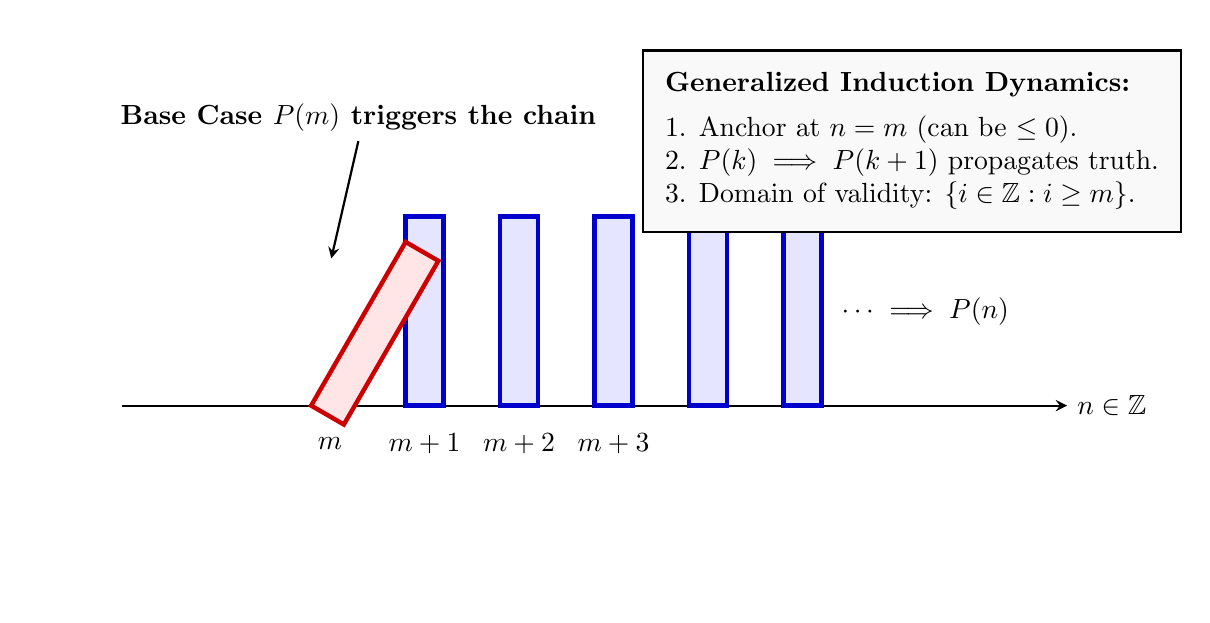
\begin{tikzpicture}[scale=1.2]
    % Layer 1: Background (White fill to ensure clean rendering)
    \fill[white] (-2,-2) rectangle (10,4);
    
    % Layer 2: Axes/Lines
    \draw[thick, ->, >=stealth] (-1, 0) -- (9, 0) node[right] {$n \in \mathbb{Z}$};
    
    % Layer 3: Plots/Shapes (Dominoes)
    % Standing dominoes
    \foreach \x in {2,3,4,5,6} {
        \draw[ultra thick, blue!80!black, fill=blue!10] (\x, 0) rectangle (\x+0.4, 2);
    }
    % Falling domino (Base case m)
    \draw[ultra thick, red!80!black, fill=red!10, rotate around={-30:(1,0)}] (1,0) rectangle (1.4, 2);
    
    % Layer 4: Nodes
    \node[black] at (1.2, -0.4) {$m$};
    \node[black] at (2.2, -0.4) {$m+1$};
    \node[black] at (3.2, -0.4) {$m+2$};
    \node[black] at (4.2, -0.4) {$m+3$};
    \node[black] at (7.5, 1) {$\dots \implies P(n)$};
    
    % Callout
    \draw[->, >=stealth, shorten >=2pt, thick] (1.5, 2.8) -- (1.2, 1.5);
    \node[black, above] at (1.5, 2.8) {\textbf{Base Case $P(m)$ triggers the chain}};
    
    % Legend (Single-Node Multiline Rule)
    \node[align=left, anchor=west, black, inner sep=8pt, draw, thick, fill=gray!5] at (4.5, 2.8) {
        \textbf{Generalized Induction Dynamics:} \\[4pt]
        1. Anchor at $n = m$ (can be $\le 0$). \\
        2. $P(k) \implies P(k+1)$ propagates truth. \\
        3. Domain of validity: $\{i \in \mathbb{Z} : i \ge m\}$.
    };
\end{tikzpicture}
\end{center}

\subsection{Heuristics \& "Cheats"}
\begin{itemize}
    \item \textbf{The "Super-Object" Cheat:} When proving a property for $n$ variables (like a product $x_1 \cdots x_n = 0$), group the first $k$ variables into a single variable $Y$. Apply the $n=2$ rule to $Y$ and $x_{k+1}$, then apply the inductive hypothesis to $Y$.
    \item \textbf{The "Add Zero" Cheat:} In divisibility proofs, if you have $A \cdot B$ and you need it to look like $C \cdot D$, try adding and subtracting a mixed term (e.g., $+ A \cdot D - A \cdot D$) to force factorization.
\end{itemize}

\subsection{Pitfalls \& Fallacies}
\begin{itemize}
    \item \textbf{The $k=1$ to $k=2$ Trap:} Assuming $P(k) \implies P(k+1)$ holds for all $k \ge 1$ without checking if the algebra actually works when $k=1$. (See Exercise 6.22, where $2k^2 \ge 2k+1$ fails for $k=1$).
    \item \textbf{Circular Reasoning:} Accidentally using $P(k+1)$ to prove $P(k+1)$. You must start with one side of the $P(k+1)$ equation and manipulate it using $P(k)$ to reach the other side.
\end{itemize}

\newpage

% ==========================================
% PART 5: CONCEPTUAL SYNTHESIS
% ==========================================
\section{Conceptual Synthesis and The "Big Picture"}

\subsection{Thematic Connections}
The central theme of this chapter is \textbf{bootstrapping truth across discrete ordered structures}. Mathematical induction unifies set theory, algebra, and logic by relying on the Well-Ordering Principle. It shows that local, microscopic rules (the transition from $k$ to $k+1$) can guarantee macroscopic, universal truths (validity for all $n \ge m$). This mirrors the concept of recursive functions in computer science, where a base return value and a recursive call define an infinite space of computations.

\subsection{Forward and Backward Links}
\begin{itemize}
    \item \textbf{Backward Links:} This topic extends foundational propositional logic. The inductive step is a formal application of \textit{Modus Ponens} applied infinitely many times: $P(m) \land (P(m) \implies P(m+1)) \vdash P(m+1)$.
    \item \textbf{Forward Links:} Understanding generalized induction is the bedrock for \textbf{Strong Induction} (where we assume $P(m) \land \dots \land P(k)$) and \textbf{Transfinite Induction} in advanced set theory (used to prove statements over uncountably infinite sets using Zorn's Lemma and ordinal numbers). In measure theory, induction is used to extend properties from algebras to $\sigma$-algebras (e.g., Carathéodory's Extension Theorem).
\end{itemize}

% ==========================================
% PART 6: ABSTRACT REAL-WORLD MODELING
% ==========================================
\section{Abstract Real-World Modeling (AI, ML, \& Quant Finance)}

\subsection{Concrete Scenarios}
\begin{enumerate}
    \item \textbf{Reinforcement Learning (Value Iteration):} In AI, proving that the Bellman operator is a contraction mapping and that Value Iteration converges to the optimal policy $\pi^*$ requires induction on the number of iteration steps $n$.
    \item \textbf{Quantitative Finance (Binomial Options Pricing):} Proving the no-arbitrage bounds of an American or European derivative on an $N$-step binomial tree requires backward induction from the terminal payoff at $t=N$ down to $t=0$.
\end{enumerate}

\subsection{Model Problem Setup: Binomial Tree No-Arbitrage Bounds}
\textbf{Context:} In Quantitative Finance, the Binomial Options Pricing Model discretizes the stochastic differential equation of an asset's price into a tree. We want to prove that the price of a European Call Option $C_0$ at time $t=0$ strictly satisfies the lower bound $C_0 \ge \max(0, S_0 - K(1+r)^{-N})$, where $S_0$ is the initial stock price, $K$ is the strike price, $r$ is the risk-free rate, and $N$ is the number of steps.

\textbf{Mathematical Formulation:}
Let the state space of the stock at step $n$ be $S_{n, j}$ for $j \in \{0, \dots, n\}$. 
The risk-neutral pricing formula states that the option price at node $(n, j)$ is:
\[ C_{n, j} = \frac{1}{1+r} \left[ q C_{n+1, j+1} + (1-q) C_{n+1, j} \right] \]
where $q \in (0,1)$ is the risk-neutral probability. The terminal payoff at step $N$ is $C_{N, j} = \max(0, S_{N, j} - K)$. Furthermore, the stock price martingale property dictates $S_{n, j} = \frac{1}{1+r} [q S_{n+1, j+1} + (1-q) S_{n+1, j}]$.

\textbf{Proof by Backward Induction on time steps $k$ (from $N$ down to $0$):}
Let $P(k)$ be the statement: $C_{N-k, j} \ge \max(0, S_{N-k, j} - K(1+r)^{-k})$ for all $j$.
\vspace{4pt} \\
\textbf{Base Case ($k=0$, i.e., $t=N$):} \\
$C_{N, j} = \max(0, S_{N, j} - K(1+r)^0) = \max(0, S_{N, j} - K)$. $P(0)$ is true by definition.
\vspace{4pt} \\
\textbf{Inductive Step:} \\
Assume $P(k)$ holds for some $k$. We evaluate $P(k+1)$, which corresponds to time $t = N - (k+1)$.
\begin{align*}
C_{N-(k+1), j} &= \frac{1}{1+r} \left[ q C_{N-k, j+1} + (1-q) C_{N-k, j} \right] \\
&\ge \frac{1}{1+r} \left[ q \max(0, S_{N-k, j+1} - K(1+r)^{-k}) + (1-q) \max(0, S_{N-k, j} - K(1+r)^{-k}) \right]
\end{align*}
Since $\max(0, x) + \max(0, y) \ge \max(0, x+y)$ and $q, (1-q) > 0$:
\begin{align*}
C_{N-(k+1), j} &\ge \max\left(0, \frac{1}{1+r} \left[ q S_{N-k, j+1} + (1-q) S_{N-k, j} - K(1+r)^{-k}(q + 1 - q) \right] \right) \\
&= \max\left(0, S_{N-(k+1), j} - K(1+r)^{-(k+1)} \right)
\end{align*}
Thus, $P(k+1)$ holds. By induction, at $k=N$ (which is $t=0$), $C_0 \ge \max(0, S_0 - K(1+r)^{-N})$. $\blacksquare$

\newpage

% ==========================================
% PART 7: COMMON VARIATIONS & UNTESTED CONCEPTS
% ==========================================
\section{Common Variations and Untested Concepts}

\subsection{Cauchy's Forward-Backward Induction}
A highly advanced variation of induction not covered in the standard homework is \textbf{Forward-Backward Induction} (or Cauchy Induction). Instead of proving $P(k) \implies P(k+1)$, we prove:
1. $P(2^k) \implies P(2^{k+1})$ (Forward step over powers of 2).
2. $P(k) \implies P(k-1)$ (Backward step to fill the gaps).

\textbf{Example: The AM-GM Inequality}
Prove that for any $n \ge 1$ positive reals, $\frac{x_1 + \dots + x_n}{n} \ge \sqrt[n]{x_1 \cdots x_n}$.
\vspace{4pt} \\
\textit{Forward Step ($n \to 2n$):} Assume true for $n$. For $2n$ variables, group them into pairs and apply the $n=2$ base case, then apply the $n$ case to the resulting $n$ terms.
\vspace{4pt} \\
\textit{Backward Step ($n \to n-1$):} Assume true for $n$. Let $x_n = \frac{x_1 + \dots + x_{n-1}}{n-1}$. Substitute this into the AM-GM inequality for $n$ variables. The algebra simplifies perfectly to yield the inequality for $n-1$ variables. This proves the theorem for all $n \in \N$.

% ==========================================
% PART 8: ADVANCED DIAGNOSTIC TESTING
% ==========================================
\section{Advanced Diagnostic Testing: "Find the Flaw"}

Below are five proofs that contain a subtle, critical logical flaw. Your task as a student is to identify the error. The solutions are provided in the key below.

\textbf{Problem 1:} Prove that all horses are the same color.
\textit{Proof:} Let $P(n)$ be the statement that in any set of $n$ horses, all horses are the same color. Base case $n=1$: A set of 1 horse trivially has the same color. Assume $P(k)$ is true. For a set of $k+1$ horses, remove the first horse; the remaining $k$ horses are the same color by $P(k)$. Put the first horse back and remove the last horse; these $k$ horses are also the same color. Since the middle horses overlap, all $k+1$ horses must be the same color. $\blacksquare$

\textbf{Problem 2:} Prove that $\sum_{i=1}^n i = \frac{n^2 + n + 2}{2}$.
\textit{Proof:} Assume $P(k)$ is true, so $\sum_{i=1}^k i = \frac{k^2 + k + 2}{2}$. For $k+1$:
$\sum_{i=1}^{k+1} i = \frac{k^2 + k + 2}{2} + (k+1) = \frac{k^2 + k + 2 + 2k + 2}{2} = \frac{(k+1)^2 + (k+1) + 2}{2}$. Thus $P(k+1)$ holds. $\blacksquare$

\textbf{Problem 3:} Prove that $x^{n-1} = 1$ for all $n \ge 1$.
\textit{Proof:} Base case $n=1$: $x^{1-1} = x^0 = 1$. Assume true for $1, 2, \dots, k$. For $k+1$: $x^{(k+1)-1} = x^k = \frac{x^{k-1} \cdot x^{k-1}}{x^{k-2}}$. By the strong inductive hypothesis, $x^{k-1} = 1$ and $x^{k-2} = 1$. Thus $x^k = \frac{1 \cdot 1}{1} = 1$. $\blacksquare$

\textbf{Problem 4:} Prove that $3^n < 2^n$ for all $n \ge 1$.
\textit{Proof:} Assume $3^k < 2^k$. Multiply both sides by $2$ to get $2 \cdot 3^k < 2^{k+1}$. Since $3^{k+1} = 3 \cdot 3^k$, and we know $2 < 3$, we can write $3^{k+1} < 2^{k+1}$. $\blacksquare$

\textbf{Problem 5:} Prove that if $A_1, \dots, A_n$ are sets, $A_1 \cup \dots \cup A_n = \emptyset \implies A_1 = \emptyset$.
\textit{Proof:} Base case $n=1$: $A_1 = \emptyset \implies A_1 = \emptyset$. Assume for $k$. For $k+1$, let $A_1 \cup \dots \cup A_{k+1} = \emptyset$. This means $(A_1 \cup \dots \cup A_k) \cup A_{k+1} = \emptyset$. By the inductive hypothesis applied to the first $k$ sets, $A_1 = \emptyset$. $\blacksquare$

\vspace{10pt}
\hrule
\vspace{10pt}
\subsection*{Solution Key: The Flaws Revealed}
\begin{enumerate}
    \item \textbf{Flaw 1 (The $k=1 \to 2$ Trap):} The inductive step fails when transitioning from $k=1$ to $k=2$. If you have 2 horses, removing one leaves a set of 1, and removing the other leaves a different set of 1. The "overlapping middle horses" set is empty, so you cannot deduce they are the same color.
    \item \textbf{Flaw 2 (Missing Base Case):} The inductive step is algebraically valid, but the base case $n=1$ yields $\frac{1+1+2}{2} = 2$, while the actual sum is $1$. A false statement can imply a false statement.
    \item \textbf{Flaw 3 (Division by Zero / Invalid Index):} The formula $x^k = \frac{x^{k-1} \cdot x^{k-1}}{x^{k-2}}$ requires $k-2 \ge 0$. When proving $P(2)$ from $P(1)$, the formula uses $x^{-1}$, which is outside the domain of the base cases established.
    \item \textbf{Flaw 4 (Inequality Direction):} The logic states $2 \cdot 3^k < 2^{k+1}$. But $3^{k+1} = 3 \cdot 3^k > 2 \cdot 3^k$. You cannot chain $3^{k+1} > 2 \cdot 3^k < 2^{k+1}$ to conclude $3^{k+1} < 2^{k+1}$.
    \item \textbf{Flaw 5 (Invalid Application of IH):} The inductive hypothesis states "If the union of $k$ sets is empty, then $A_1$ is empty." In the $k+1$ step, we know $(A_1 \cup \dots \cup A_k) \cup A_{k+1} = \emptyset$, which implies $(A_1 \cup \dots \cup A_k) = \emptyset$. The proof skips this deduction and blindly applies the IH without justifying that the premise of the IH was met.
\end{enumerate}

\end{document}